\section{Overview\label{overview}}


\begin{figure}[h]
    \centering
    \vspace{-0.4cm}
    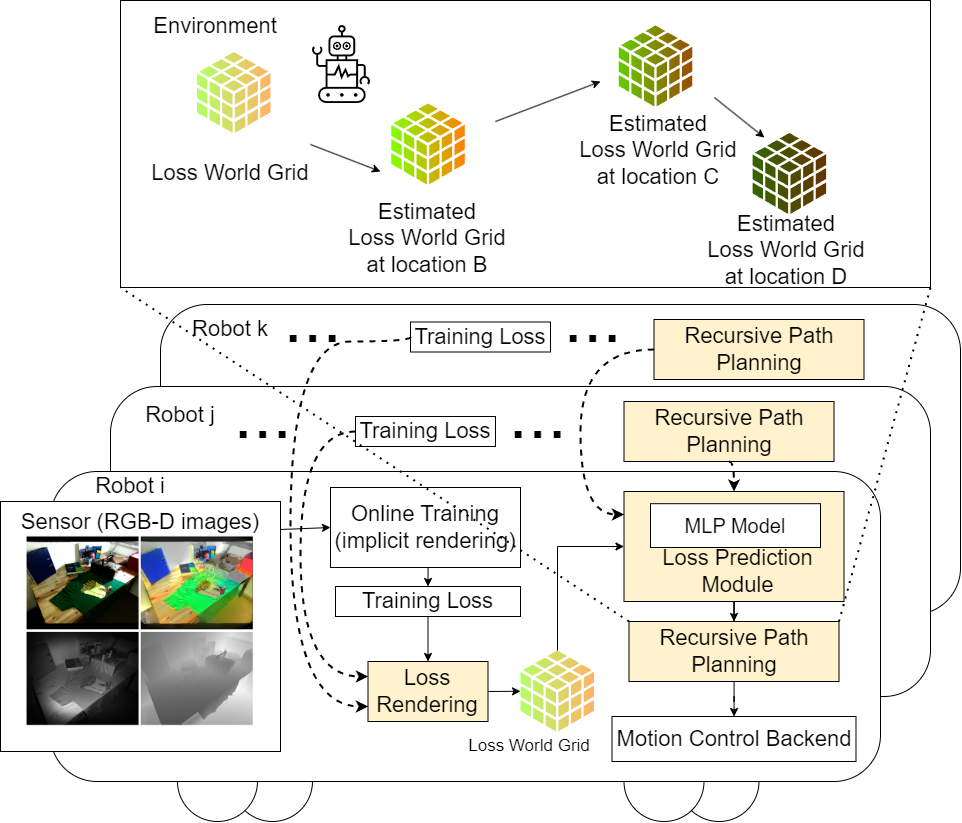
\includegraphics[width=\linewidth]{fig/overview.drawio.png}
    \caption{Overview of LODA.% During training of the online training task, training loss is exchanged and rendered to a Loss World Grid, which is used to train an MLP model that learns the loss dynamics of the Loss World Grid and is used to recursively predict the future state of the Loss World Grid in recursive path planning. The planned paths from other robots are also used to predict the future state of the Loss World Grid as the basis of local recursive path planning.
    }
    \label{fig:overview}
    \vspace{-0.5cm}
  \end{figure}


  % \begin{figure*}[t]
  %   %\vspace{-0.6cm}
  %   \centering
  %   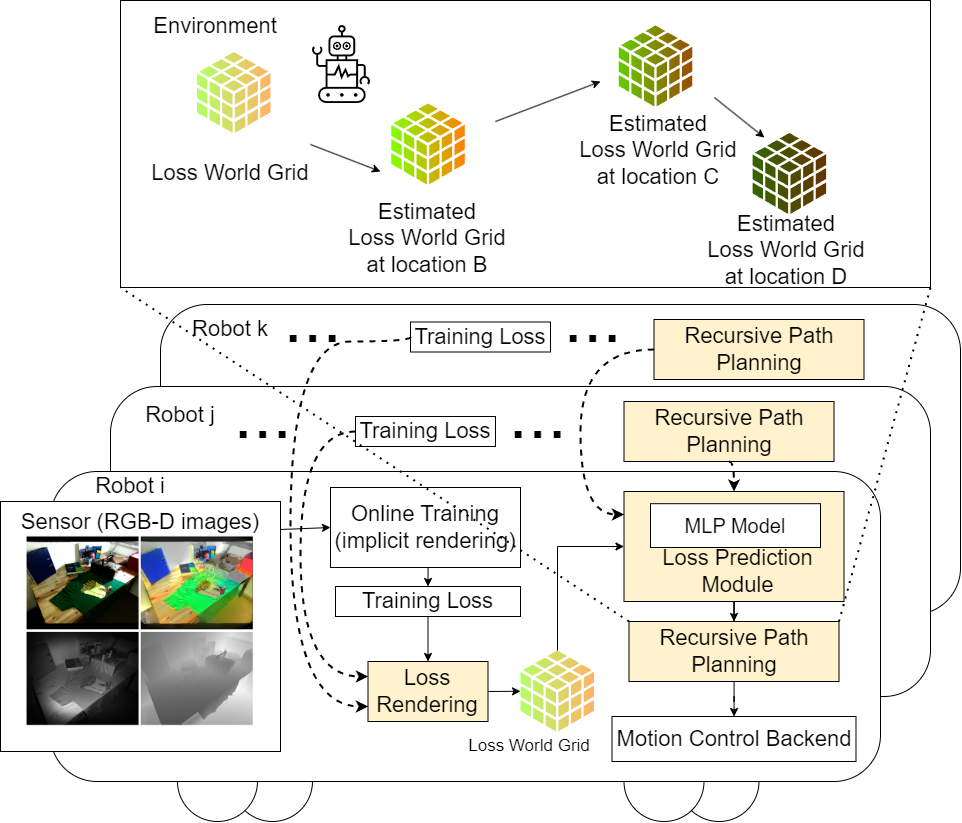
\includegraphics[width=0.98\linewidth]{fig/overview.drawio.png}
  %   \caption{New Overview of MIAS}
  %   % \label{fig:overview}
  %   %\vspace{-0.3cm}
  % \end{figure*}


% This chapter presents the architecture of LODA and gives an overview of how LODA models the loss dynamics of the environment and how it is used to search for path with optimal accumulated information gain with a single robot or the cooperation of multiple agents in the LODA-RPP algorithm.

As shown in Fig.~\ref{fig:overview}, assume that each robot is a four-wheel robot with sensors (e.g., cameras, lidar) attached to it and it is periodically taking samples ($I_i \in \bm{I}$) from the sensors as the training input for an underlying online training task (e.g., 3D reconstruction), where $i=1,2,\dots$ means the $i^{th}$ sample and $\bm{I}$ is the sample space of the environment.
We assume that the size of the environment is limited and navigable for the robot, such as a room or an office.
The underlying online training task trains an AI model $\theta$ periodically on collected training input to extract knowledge (e.g., increase in accuracy of the AI model) from the environment and $L(\theta_t, I_i)$ is the training loss function on sample $I_i$ at time $t$.
The goal of automatic high quality training data acquisition for a such scenario is 

\begin{equation}
  \begin{aligned}
    \vspace{-0.5cm}
    \mathop{\min} & \quad t, m \\
    \mathop{s.t.} & \quad L(\theta_t)\approx \frac{1}{m} \sum_{i=1}^{m} L(\theta_t, I_i) < t_{loss} \\
      & \quad C(\{I_i\}) > t_{coverage}
  \end{aligned}
  \label{mini1}
\end{equation}
where $C(\cdot)$ is the coverage estimation of the samples.
It means finding a minimum sequence of samples that fastest covers the environment and have the highest information gain to reduce the loss function which forms the navigation path of the robots.
% While the fast coverage problem is well approximated by traditional RRT algorithms, we aim at approximating the problem of finding a navigation path for the robot to acquire the sequence of ${I_i}$ of highest information gain in this paper.
% We are aiming to find a navigation path for each robot to optimize quality of the collected training data so that the online training task can achieve high performance (e.g., overall loss function $L(\theta_n)$ lower than a threshold $t$) within as short as possible time (thus as few as possible training iterations and training input): 

% \begin{equation}
  %   \begin{aligned}
    %     \mathop{\min} & \quad n, m \\
    %     \mathop{s.t.} & \quad L(\theta_n) < t \\
    %   \end{aligned}
    %   \label{mini}
    % \end{equation}
    
% The fact that $\theta_t$ is varying over time invalidates the methods that statically consider the model $\theta$ and we explore the dynamic metrics of the training model and come into loss dynamics.
Considering the evolution of $\theta$ over time, the variation of $\theta_t$ is typically impossible to predict. % and thus we we cannot extend the active learning methods to predict the future $I_{i+1}$ with highest information gain when we have predicted $I_{i}$ for the current model.
Instead, we predict the level of information gain when $I_{i}$ is acquired exploiting loss dynamics through the following components of our system: loss rendering, loss dynamics modelling and future loss prediction, and finally forms an optimal path with recursive path planning as discussed below.

\vspace{-0.5cm}
\subsection{Loss Prediction Module}
In LODA, we store the running statistics of training loss by rendering it to a sparse grid of tensor named World Loss Grid (WLG) in correspondence to the coordinates of the training samples in the environment.
An MLP model is periodically trained based on these data to learn the dynamics of loss and predict future loss given a desired sampling position and orientation.
The MLP model is online trained to adapt to possible different loss intensity and different loss dynamics in different environments or online training tasks.

% In LODA, based on the Loss Prediction Module, we predict the future training loss when the training AI model is trained on newly collected data and calculate loss reduction as an approximation of possible information gain (discussed in detail in the next section) for recursive path planning.
% To predict such loss reduction for path planning on every robot, we periodically sample and distribute the training loss among all robots.
% The loss and extra information such as its average, weight (times visited), the sampling position and orientation of the training data are then rendered and stored in a sparse grid of tensor named World Loss Grid, which is in correspondence to the environment.
% An MLP model is periodically trained based on data on the grid to predict future loss given a desired sampling position and orientation and the corresponding tensors (selected by frustum selection) on the sparse grid, which is the basis for information gain estimation.
% The MLP model is online trained to adapt to possible different loss intensity and different loss dynamics in different environments or online training tasks.

% Since this prediction of training loss from has the same meaning of the input data for prediction from the sparse grid, which is also loss, the prediction result can be merged back to the sparse grid for the prediction when searching for the next step in a recursive way.

\vspace{-0.5cm}
\subsection{Recursive Path Planning}
% Since it is impractical to search all possible paths even in an environment with limited size,
% we integrate our path planning with RRT* algorithm which searches obstacle-free paths in width-first style and recursively estimate the accumulated information gain.
As in Fig.~\ref{fig:overview}, starting from the original WLG, we predict the training loss when a next step is taken using the loss prediction module (excluded for simplicity in the figure) and incrementally render a new sparse grid,.
On the basis of the predicted new sparse grid, we continue to predict the training loss for the following steps recursively and finally at the end of the path the accumulated information gain estimation of the whole path is calculated as the difference between the final predicted sparse grid and the original to search for the path with optimal accumulated information gain.
% With the estimation results of the candidate paths, the path with the highest potential accumulated information gain can be found.

To support multi-robot cooperation in active high quality training data acquisition, a robot should consider the plans from other robots and estimate the impact of the plans from other robots for the decision making of itself.
In LODA this can be easily achieved with the above design.
We recursively predict the resulting sparse grid of training loss of planned paths from other robots and merge it with the original WLG as the basis of recursive path planning of this robot, resulting in a cooperative path considering the impact from the possible actions from other robots.



